67. \begin{figure}[ht!]
\center{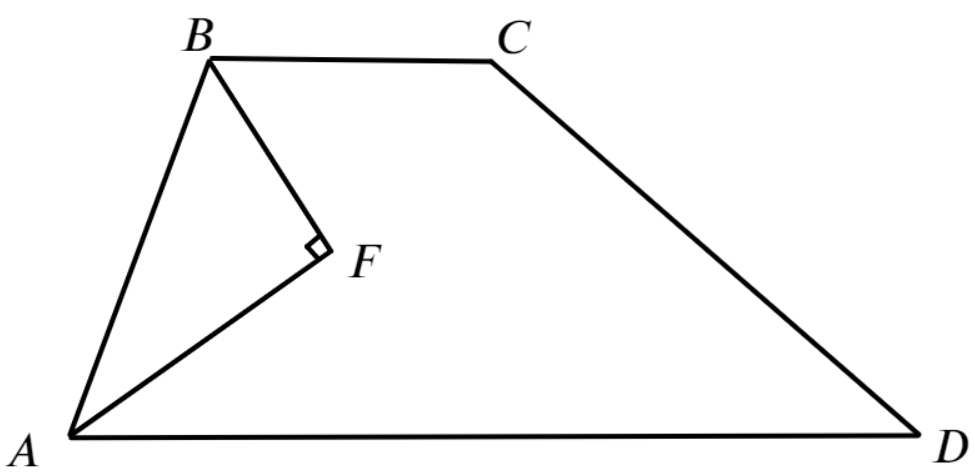
\includegraphics[scale=0.35]{g9-67.png}}
\end{figure}\\
Углы $A$ и $B$ являются односторонними, значит $\angle A+\angle B=180^\circ,$ поэтому $\angle BAF+\angle ABF=\cfrac{1}{2}(\angle A+\angle B)=90^\circ$ и $\angle AFB=180^\circ-90^\circ=90^\circ.$ Тогда по теореме Пифагора получаем $AB=\sqrt{24^2+10^2}=26$см.\newpage\noindent
